%% LyX 2.1.4 created this file.  For more info, see http://www.lyx.org/.
%% Do not edit unless you really know what you are doing.
\documentclass[12pt]{scrartcl}
\usepackage{lmodern}
\usepackage{lmodern}
\usepackage[T1]{fontenc}
\usepackage[latin9]{inputenc}
\usepackage{geometry}
\geometry{verbose,bmargin=1.5cm,lmargin=1.5cm,rmargin=1.5cm}
\usepackage{amsmath}
\usepackage{amssymb}
\usepackage{graphicx}
\usepackage{setspace}
\usepackage{wasysym}
\usepackage[authoryear]{natbib}
\doublespacing

\makeatletter

%%%%%%%%%%%%%%%%%%%%%%%%%%%%%% LyX specific LaTeX commands.
\newcommand{\lyxmathsym}[1]{\ifmmode\begingroup\def\b@ld{bold}
  \text{\ifx\math@version\b@ld\bfseries\fi#1}\endgroup\else#1\fi}

%% Because html converters don't know tabularnewline
\providecommand{\tabularnewline}{\\}

%%%%%%%%%%%%%%%%%%%%%%%%%%%%%% Textclass specific LaTeX commands.
\newcommand{\lyxaddress}[1]{
\par {\raggedright #1
\vspace{1.4em}
\noindent\par}
}

\@ifundefined{date}{}{\date{}}
%%%%%%%%%%%%%%%%%%%%%%%%%%%%%% User specified LaTeX commands.
\usepackage{lineno}

\makeatother

\begin{document}

\title{{\large{}Eco-evolutionary diversification of trait convergence and
complementarity in mutualistic networks }}


\author{{\normalsize{}Francisco Encinas-Viso$^{1,*}$, Rampal S. Etienne$^{2,**}$
and Carlos J. Meli�n$^{3,**}$}}

\maketitle

\lyxaddress{\textbf{\medskip{}
}\\
 \textbf{1}) NRCA \& Centre for Australian National Biodiversity Research,
CSIRO, GPO Box 1600 Canberra , Australia \\
 \textbf{2}) Groningen Institute for Evolutionary Life Sciences, University
of Groningen, The Netherlands \\
 \textbf{3}) Department of Fish Ecology and Evolution, Center for
Ecology, Evolution and Biogeochemistry, EAWAG, Swiss Federal Institute
of Aquatic Science and Technology, Switzerland\medskip{}
\\
 Keywords: Diffuse coevolution, specialization, sexual reproduction,
assortative mating, dispersal limitation, phylogenetic relatedness,
obligate mutualism, morphological constraints, individual based model.\medskip{}
\\
 Type of Article: Letters\\
 Number of figures: 7 (6 in color); Number of tables: 1\\
 {*} Corresponding author: franencinas@gmail.com\\
 {*}{*} Joint last authorship}

\begin{linenumbers}

\newpage{} 
\begin{abstract}
Empirical mutualistic networks composed by several interacting species
show high levels of trait convergence and complementarity. Convergence
and complementarity have been attributed to coevolutionary selection
coming from both plant and animals, selection coming only from the
mutualistic partners and also due to niche-based processes. Non-selective
causes like traits evolving due to a Brownian motion can also produce
evolutionary trait convergence and complementarity. Whether coevolutionary
selection or non-selective causes are required to explain trait convergence
and complementarity, the impact of population, trait and diversification
dynamics on quantitative trait divergence and convergence dynamics
in species-rich mutualistic networks remains largely unexplored. Here,
we present a landscape genetics model to connect population, trait
and diversification dynamics to study complementarity, convergence
and nestedness in species-rich mutualistic networks. We compare our
model to convergence and complementarity patterns observed in a plant-hummingbird
mutualistic network to show that population, trait and diversification
dynamics predict well plant-animal complementarity and convergence
for animals but not for plants. Our analysis also shows that high
levels of convergence, complementarity and nestedness are possible
to predict after controlling by phylogenetic relatedness. Our results
demonstrate that, in contrast to previous models based on coevolutionary
selection, diversification trait dynamics requires ecological (demography
and dispersal limitation), genetical (mutation, recombination and
assortative mating), and morphological processes associated to trait
matching to reproduce key patterns of mutualistic networks, from trait
convergence and complementarity to nestedness. \newpage{}
\end{abstract}

\section*{Introduction}

Since Darwin's book ``On The Origin of Species'' \citep{darwin_origin},
the idea of coevolution, defined as reciprocal evolutionary trait
change between species, has sparked interest from biologists trying
to understand how species interactions generate trait changes. The
first clear indication of coevolution was Darwin's moth example \citep{Darwin_orchids_book}
showing that the long corolla from the orchid \emph{Angraecum sesquispedale}
could only be reached by a pollinator species with a similar or larger
proboscis length. Following the moth and orchid mutualism model system,
several studies have modeled coevolutionary dynamics of a few species
\citep{Ferriere-2007,Law2001,Ferdy_2002,Gomulkiewicz-2003,Jones_Ferriere_amnat_2009},
particularly highly specialized (i.e. obligatory mutualists) systems
of plant-animal interactions, such as the fig-fig wasp mutualism \citep{Bronstein-2006}.
These studies have determined the ecological conditions for coevolutionary
stable systems in highly specialized plant-animal interactions \citep{Law2001,Jones_Ferriere_amnat_2009}.

\citet{Janzen_coevolution_1980} argued that high specialization between
plants and animals was not the only example of coevolution, but coevolution
can also be the product of multiple-species interactions, a term that
he coined ``diffuse coevolution''. Diffuse coevolution means that
selection on traits is determined by the interaction of more than
two species and not only based on pairwise interactions. This is based
on the idea of pollination or dispersal ``syndromes'', where plants
have a set of traits that attract a specific group of pollinator or
animal seed-disperser species with traits complementary to those of
the plants. The idea of ``diffuse coevolution\textquotedblright{}
is thus linked to concepts of complementarity and convergence, and
has also been related to patterns of nestedness detected across biogeographic
regions in mutualistic networks. 

Nestedness, defined as a non-random pattern of interactions where
specialist species interact with proper subsets of more generalist
species introduces the concept of ``diffuse coevolution\textquotedblright{}
in a more quantitative context \citep{Bascompte-2003}. Patterns of
nestedness have been shown to provide information about the underlying
network dynamics. For example, nestedness may be associated with stability
and coexistence of species in mutualistic networks \citep{Bastolla2009,Okuyama-2008},
although these properties might be also independent of nestedness
(Pitchford \& Plank 2012).

Complementarity, trait matching between mutualistic partners (e.g.
corolla length-proboscis length, frugivore body mass-seed size, \citep{Bascompte-Jordano-2007})
could be the product of reciprocal evolution (i.e. coevolution). In
highly specialized two-species interactions, as for example the fig-fig
wasp mutualism \citep{Bronstein-2006}, plants coevolve with their
most efficient pollinator to strengthen the complementarity of their
matching adaptations (i.e., coevolutionary selection). There are also
situations where an insect will be unable to reach nectar in floral
tubes longer than its proboscis: the tube length sets up a barrier
to some species, but not to others. For example, combining rules that
link plants to pollinators whose trait ranges overlap and rules that
link pollinators to flowers whose traits are below a pollinator-specific
barrier value seem to predict structural properties of empirical mutualistic
networks \citep{SantamariaRodriguez2007}. Thus, developmental and
morphological constraints may be required to explain complementarity
\citep{Bascompte-Jordano-2007,Andersonetal2010}.

Convergence, the independent evolution of similar features in the
same community in different evolutionary lineages is a common, perhaps
a ubiquitous phenomenon but its interpretation is not clear-cut \citep{Losos_2011}.
Selective and non-selective causes can produce evolutionary trait
convergence \citep{Losos_2011}. Traits may evolve according to the
same environmental or biotic pressures in independent lineages or
as Brownian motion with speciation occurring randomly \citep{Stayton_2008}.
Evolutionary convergence in plant-animal mutualisms partly explains
the formation of 'syndromes' produced by the presence of specific
mutualist partner species \citep{Waser_1996,Howe_1982,Bascompte-Jordano-2007}.
For example, plant species with a specific corolla morphology may
determine the evolutionary convergence of pollinator species traits
\citep{Jousselin_2003,guimaraes_coevol_2011}.

Recently, \citet{guimaraes_coevol_2011} and \citet{Nuismeretal2012}
explored evolutionary models using a broad range of coevolutionary
selection values to study convergence and complementarity in mutualistic
networks. \citet{guimaraes_coevol_2011} show that convergence in
a one-dimensional trait within a trophic level may in part emerge
as a consequence of selection for a complementarity trait between
trophic levels. For weak or absent coevolutionary selection, \citet{Nuismeretal2012}
show that trait values in animal and plant species can be highly variable
and non-convergent but positively correlated (i.e., complementary).
As coevolutionary selection intensifies, variation in the trait values
of animal and plant species is reduced and convergence emerges but
correlations between traits of interacting species are weakened (i.e.,
low pairwise complementarity). \citet{Nuismeretal2012} further explored
the connection between convergence and complementarity to nestedness
patterns in mutualistic networks. They showed that interactions mediated
by a mechanism of phenotype matching tend to be antinested when coevolutionary
selection is weak and become even more strongly antinested with increasing
coevolutionary selection favoring the emergence of reciprocal specialization.
Taken together, these results suggest that it is not trivial to explain
simultaneously a high degree of convergence, complementarity and nestedness
in species-rich mutualistic networks as observed the empirical data.

Difficulties in obtaining predictions of simultaneously large values
of convergence, complementarity and nestedness in mutualistic networks
may also be a consequence of unexplored drivers currently lacking
in models of mutualistic networks. Most ecological models have focused
on population dynamics to study nestedness while evolutionary models
have focused on trait-based dynamics of interacting species, particularly
the emergence of complementarity and convergence in the absence of
population dynamics \citep{Nuismer2004,KokkoLopezSepulcre2007,Bascompte-Jordano-2007,guimaraes_coevol_2011,Nuismeretal2012}.
However, demography and trait evolution may interact to produce feedbacks
and eco-evolutionary dynamics (\citet{Schoener2011}). Yet, eco-evolutionary
spatial diversification models combining simultaneously population
and trait dynamics to connect trait-based patterns as complementarity
and convergence with nestedness in mutualistic networks are currently
lacking. 

Much work on diversification emphasizes on ecological divergence and
speciation \citep{Schluter:2009,Doebeli_book,Seehausenetal_2014,Rainey_Travisano:1998,Butlin_Bridle_Schluter_2009,Gavrilets_Losos_2009},
but we propose here to step back and ask basic questions about the
dynamics of divergence in mutualistic networks, and how it may depend
on sexual reproduction, spatial, genetic, morphological and demographic
processes. Before we understand the full impact of adaptation, coevolutionary
selection and ecological speciation on evolution and diversity in
ecologically complex mutualistic networks, we need to understand well
the basic dynamics of mutation, gene flow, drift, morphological and
spatial constraints underlying the process of diversification in species-rich
mutualistic networks. Thus, to further understand the trade-offs between
convergence, complementarity and nestedness in mutualistic networks,
diversification models accounting for phylogenetic relatedness combining
demographic, morphological constraints and evolutionary processes
of trait divergence and convergence in species-rich mutualistic networks
are required. Here, we extend landscape genetics models of diversification
dynamics that combine evolutionary forces (mutation, recombination
and genetic drift, \citep{kimura,hubbell_book,Lynch_2007,Vellend2010})
with demographic processes (migration, ecological drift, speciation
and extinction, \citep{Gavriletsetal2000,deaguiar_2009,melian_2012,Higgs_Derrida:1992})
to connect quantitative trait dynamics in sexually reproducing plant
and pollinator populations to convergence, complementarity and nesstedness
in mutualistic networks.

We find that diversification dynamics change trait distributions,
and patterns of convergence, complementarity, nestedness and connectance
in mutualistic networks. We show that convergence and complementarity
emerge together with high levels of nestedness in the absence of coevolutionary
selection. Our model predcits that trait convergence occurs mostly
between the common species and on average in approximately $20\%$
of all possible events while trait complementarity occurs in approximately
$30\%$ of all possible events. Our model predicts well plant-animal
complementarity and convergence for animals but not for plants in
a empirical plant-hummingbird mutualistic network. In contrast to
previous studies where interactions mediated by a mechanism of phenotype
matching tended to be antinested when coevolutionary selection was
weak, we found that, in the absence of coevolutionary selection, highly
nested values are obtained in agreement with the empirical mutualistic
networks. Taken together our results suggest that diversification
dynamics combining ecological (demography and dispersal limitation),
population genetics (mutation, recombination, assortative mating and
drift) and morphological constraints associated to trait matching
expand theoretical approaches to predict the key patterns of mutualistic
networks, from trait convergence and complementarity to connectance
and nestedness.


\section*{{\large{}The model: Eco-evolutionary diversification in mutualistic
networks}}

We consider a landscape consisting of several individual plants (\emph{P})
and animal pollinators (\emph{A}). Individuals belonging to these
two communities interact mutualistically and we assume obligate mutualism
for both partners. Furthermore, the number of individuals at each
trophic level is fixed and equal to the environmental carrying capacity
for the given community. Genetic, phenotypic and species composition
change in time and space due to replacement of dead individuals by
offspring of the same or another species (the key terms and model
steps are summarized in figure \ref{fig:Recombination} and table
1, respectively). In this section we explain how we model population,
diversification and trait dynamics.


\subsection*{\textmd{Population dynamics }}

Our model is a stochastic individual-based model with overlapping
generations. The population consists of $J_{P}$ and $J_{A}$ haploid
gonochoric (i.e. separated sexes) individuals with an explicit genome
of size $L$ each and equal sex ratios at the outset. The genome of
each individual is composed by $L-1$ assortative mating loci and
one neutral locus. Both plant and animal population reproduce sexually
and are spatially structured. Demography follows by randomly selecting
to die an individual plant $k$ and animal $k'$. There are four conditions
for producing viable offspring for the plant and animals, concerning:
1) geography, 2) genetics, 3) obligate mutualism and 4) morphology: 
\begin{enumerate}
\item Geography: a female and a male individual within the plant and animal
populations are randomly chosen among all females and males within
a distance $d_{max}$ of the dead plant $k$ and dead animal $k'$
. This requires two geographic distance matrices, one for plants,
$D^{P}$ = {[}$d_{ij}^{P}${]}, and one for animals, $D^{A}$ = {[}$d_{ij}^{A}${]},
containing all the pairwise distances. 
\item Genetics: to produce a viable offspring between the female and the
male in the plant and animal populations, they must have a genetic
similarity value of the assortative mating loci, $q_{\venus\mars}$,
higher than the minimum genetic similarity to have viable offspring,
$q_{min}$, ($q_{\venus\mars}>q_{min}$). This process reflects assortative
mating and it requires two genetic similarity matrices, one for plants,
$Q^{P}$ = {[}$q_{ij}^{P}${]}, and one for animals, $Q^{A}$ = {[}$q_{ij}^{A}${]},
containing all the pairwise similarity values. 
\item Obligate mutualism: that the geographic distance between the female
$\venus$ (animal or plant) and one of the two male animal or plant
individuals, represented here as $j$, is lower than the maximum distance,
$d_{max}^{PA}$, ($d_{j\venus}^{PA}<d_{max}^{PA}$). This requires
one geographic distance matrix, $D^{PA}$ = {[}$d_{ij}^{PA}${]},
containing all the pairwise distances. 
\item Morphology: female plants need the presence of an animal pollinator
with a larger or equally-sized proboscis than the corolla of the female
plant, thus the phenotype of the selected pollinator, represented
here as $j$, must satisfy $z_{\venus}^{P}\leq z_{j}^{A}$. This requires
two phenotype distributions, one for the plants, $Z^{P}=[z_{i}^{P}]$
and one for the animals, $Z^{A}=[z_{i}^{A}]$. This mechanism is similar
to the the ``phenotypic difference'' mechanism assumed in the model
of \citet{Nuismeretal2012}. 
\end{enumerate}
The offspring arising from this mating event will occupy the geographic
position of the just deceased individual.


\subsection*{\textmd{Diversification dynamics}}

To quantify speciation events we calculate the genetic distance between
each pair of individuals based on the assortative mating loci. We
represent the genome of each individual by a sequence of $L-1$ loci,
where each locus can be in two allelic states, $+1$ or $-1$. The
assortative mating loci of each plant individual $i$ in a population
of size $J_{P}$ is represented as a vector: $S^{i}=(S_{1}^{i},S_{2}^{i},...,S_{L}^{i})$,
where $S_{u}^{i}$ is the $u^{th}$ locus of individual $i$. The
genetic similarity based on assortatove mating loci between individuals
$i$ and $j$ is calculated as the sum of identical loci across the
genome

\begin{equation}
q_{ij}^{P}=\frac{1}{L}\sum_{u=1}^{L}S_{u}^{i}S_{u}^{j}\label{eq:genetic_similarity}
\end{equation}
where $q_{ij}^{P}\in\{-1,1\}$ with the genetic similarity matrix,
$Q^{P}$ = {[}$q_{ij}^{P}${]}, containing all pairwise genetic similarity
values for plants (the same for animals, $Q^{A}$ = {[}$q_{ij}^{A}${]}).
The genome of the offspring is obtained by a block cross-over recombination
of a female genome, $S^{\venus}$, and a male genome, $S^{\mars}$,
where a locus $l$ in the genome of the parents is randomly chosen
partitioning the genome of each individual in two blocks. All genes
beyond that locus $l$ in either genome are swapped between the two
parents and eventually form two new genomes. One of the two new genomes
is randomly chosen for the offspring. The offspring's genome undergoes
mutations at mutation rate $\mu$. Figure \ref{fig:Recombination}
describes the recombination-mutation process.

At the beginning of the simulations all individuals are genetically
identical (all $q_{ij}^{P}$ and $q_{ij}^{A}$ = 1); hence they are
all able to mate and produce viable offspring. The genetic similarity
between individuals of a guild can be visualized as an evolutionary
spatial graph \citep{melian2010_plos}, where nodes correspond to
individuals and the edges correspond to the geographic distances between
a pair of individuals satisfying the genetic similarity condition
for mating, $q_{ij}^{P}(q_{ij}^{A})>q_{min}$. The connectance of
the graph will decrease when generations move forward because of the
processes described in the previous section: 1) spatial constraints
for mating driving assortative mating and dispersal limitation; 2)
genetic divergence driven by the threshold for mating (incompatibilities),
mutation and recombination forming the genome of the offspring; 3)
obligate mutualistic interactions driven by spatial proximity of individuals
of the other guild, and 4) morphological constraints.

These four set of processes drive genetic divergence and speciation.
We followed the species definition of \citet{Nei1983}, which states
that species are groups of individuals that are reproductively isolated
and can interbreed to produce fertile offspring. In our model this
is realized through allowing two individuals to mate successfully
if their genetic similarity value is larger or equal to the minimum
value, $q_{min}$. Thus, speciation is defined as a group of genetically
related individuals, where two individuals in a sexual population
can be conspecific while also being incompatible, as long as they
can exchange genes indirectly through other conspecifics \citep{deaguiar_2009,melian2010_plos}.
This is the definition of 'ring species' \citep{MoritzSchneider1992}.

Genetic divergence will eventually produce the formation of two genetically
incompatible clusters of individuals, i.e. two species. This speciation
process, also called 'fission-induced' speciation, continues to form
more clusters and genetic divergence between individuals of different
species increases. However, the diversification dynamics will fluctuate
due to random extinctions (death of last individual of a species).
A stochastic balance between speciation and extinction is eventually
reached giving the final steady-state of the metacommunity.


\subsection*{\textmd{Quantitative trait dynamics}}

We model each individual plant and animal with a quantitative trait,
$z^{P}$ and $z^{A}$, respectively. The processes described in figure
\ref{fig:Recombination} govern two quantitative traits, one for each
guild: proboscis or bill length ($z_{i}^{A}$) in pollinators and
corolla length ($z_{i}^{P})$ in plants. The quantitative trait of
offspring is determined by the additive genetic effects of the genome
(i.e. no epistasis) after the process of randomly choosing one of
the new two genomes and mutation (figure \ref{fig:Recombination})
plus a normally distributed environmental effect, $\epsilon$, $\mathcal{N}(\mu_{\epsilon}=0,\sigma_{\epsilon}^{2}=1$)
\citep{guimaraes_coevol_2011}. The phenotype of the plant offspring
$i$ is $z_{i}^{P}=g_{i}^{P}+\epsilon$ and the genetic component
($g_{i}^{P}$) of the phenotype of offspring $i$ is

\begin{equation}
g_{i}^{P}=L+S_{o}^{i}\label{eq:genetic_comp}
\end{equation}
with $S_{o}^{i}=\sum_{u=1}^{L}S_{u}^{i}$. Hence $g_{i}^{P}$ is calculated
as the sum of alleles across the genome \citep{kondrashov_shpak_1998}
plus the number of loci to avoid negative trait values ($g_{i}^{A}$
is calculated similarly for animals). We assumed that the magnitude
of the influence (i.e., effect sizes) of any given locus on this quantitative
trait is equal across all the loci \citep{Seehausenetal_2014}. This
means that two individuals with a different combination of alleles
in the genome can express the same quantitative trait \citep{Losos_2011}.


\subsection*{\textmd{Neutral locus evolution}}

We considered a neutral locus to estimate genetic divergence among
species for the calculation of convergent events (see section ``Evolutionary
convergence''). The neutral locus is located at the end of the genome
at the position $L$ and has $k$ possible allelic states. The locus
is completely unlinked from the rest of the genome that contains the
assortative mating loci. We used low mutation rates for this neutral
locus, $\mu_{neutral}=10^{-7}$ , and the $k$ allele mutation model
(i.e. model in which each allele can mutate to any of the other $k\lyxmathsym{\textendash}1$
possible alleles with equal probability (\citet{Hobanetal2013}).
We used the Cavalli-Sforza distance to calculate the matrix of genetic
distances among species (\citet{CavalliEdwards1967}).


\section*{{\large{}Convergence, complementarity and nestedness}}


\subsection*{\textmd{Evolutionary convergence}}

The calculation of convergence requires computing pairwise genotypic
and phenotypic similarities and the similarity between mean species
phenotypes from distantly related species. With only three species,
only one convergence is possible after excluding the sister species
(see figure \ref{fig:Evolutionary-convergence}). The number of convergences
potentially increases with the number of species present. For example,
if we have ten species and we exclude one of them as the sister species
of the focal species, we have nine species to calculate convergence.
If we find that two out of nine species are phenotypically similar
enough to the focal species, we count two (out of nine,$\sim22\%$)
convergences. We repeat this by changing the focal species and calculate
the mean convergence events over all species. In contrast to previous
approaches that used the mean pair-wise difference between traits
of species \citep{guimaraes_coevol_2011} or the variance of species
traits in a guild as a proxy to predict convergence (i.e., large values
weak convergence whereas small values of the variance may indicate
strong convergence, \citep{Nuismeretal2012}), we used the relationship
between genetic divergence and phylogenetic relatedness for the estimation
of evolutionary convergences. The advantage of our method considering
phylogenetic relatedness is that it excludes cases of development
of very similar trait values from sister species (i.e., parallel evolution,
\citep{Losos_2011}) and therefore it does not overestimate convergence
events. Finally, to visualize the genetic relatedness between species
we constructed clustering trees using Euclidean distance with the
Python library ETE 2.01 \citep{ete_python}).


\subsubsection*{\textmd{Phenotypic similarity}}

The phenotypic similarity for plants ($p_{ij}^{P}$) between individual
$i$ and $j$ is defined as 
\begin{equation}
p_{ij}^{P}=1-\frac{|z_{i}^{P}-z_{j}^{P}|}{z_{max}^{P}}\label{eq:phenotypic_sim}
\end{equation}
where $z_{i}^{P}$ and $z_{j}^{P}$ are the phenotypic similarity
values of $i$ and $j$, respectively, and $z_{max}^{P}$ is the maximum
value of the phenotype distribution, $Z^{P}$ . Thus, the elements
$p_{ij}^{P}\in\{0,1\}$ of the phenotypic similarity matrix, $\mathcal{P}^{P}$
= {[}$p_{ij}^{P}${]} represent all pairwise values for plants (the
same for animals, $\mathcal{P}^{A}$ = {[}$p_{ij}^{A}${]}).


\subsubsection*{\textmd{Mean genetic and phenotypic species similarity}}

We define evolutionary convergence as the similarity between average
species phenotypes from distantly related species. We assume that
two species are distantly related, in phylogenetic terms, if they
do not come from a direct common ancestor, i.e. they are not sister
species. To exclude sister species from the analysis we need to calculate
the mean genetic similarity among species of the same guild. The mean
genetic similarity between a plant species $k$ and a plant species
$l$ is

\begin{equation}
\hat{q}_{kl}^{P}=\frac{1}{n_{k}n_{l}}\sum_{i=1}^{n_{k}}\sum_{j=i}^{n_{l}}q_{ij}^{P}\label{eq:genetic_sim_species}
\end{equation}
where $q_{ij}^{P}$ is the genetic similarity between an individual
$i$ of plant species $k$ and an individual $j$ of plant species
$l$, and $n_{k}$ and $n_{l}$ are the absolute abundances of plant
species $k$ and $l$, respectively. The elements $\hat{q}_{kl}^{P}$
form the matrix $Q_{s}^{P}=[\hat{q}_{kl}^{P}]$ from which the sister
species of each species in the guild can be identified (The elements
for animals, $Q_{s}^{A}=[\hat{q}_{kl}^{A}]$, are calculated in the
same way as we did for the plants). To calculate evolutionary convergence
we need to know the average phenotypic similarity between two species.
We define phenotypic similarity between species $k$ and $l$ as

\begin{equation}
\hat{p}_{kl}^{P}=\frac{1}{n_{k}n_{l}}\sum_{i=1}^{n_{k}}\sum_{j=i}^{n_{l}}p_{ij}^{P}\label{eq:phenotypic_sim_species}
\end{equation}
which is analogous to the definition of eq. \ref{eq:genetic_sim_species},
but now considering phenotypes instead of genotypes. This will build
a species phenotypic similarity matrix $P_{s}^{P}=[\hat{p}_{kl}^{P}]$
(the species phenotypic similarity matrix, $P_{s}^{A}=[\hat{p}_{kl}^{A}]$,
is calculated analogously for the animals). We then focus on each
species in turn and exclude its sister species to avoid cases of parallel
evolution to calculate the number of convergences related to the focal
species. We define a focal plant species $k$ and a non-sister plant
species $l$ to be convergent if phenotypic similarity between them
is higher than between focal and sister species ($\hat{p}_{k,sister}^{P}<\hat{p}_{kl}^{P}$)
and higher than a certain phenotypic threshold value $t_{conv}$ ($\hat{p}_{kl}^{P}>t_{conv})$;
convergent species is calculated analogously for the animals).


\subsection*{\textmd{Evolutionary complementarity}}

Evolutionary complementarity does not require the genetic similarity
matrix. We only need to estimate the phenotypic similarity between
plant and animal species and we do this as we did for the evolutionary
convergence. We calculate the phenotypic similarity matrix $P_{s}^{PA}=[\hat{p}_{kh}^{PA}]$.
This matrix contains the mean trait similarity for each plant species
$k$ and animal species $h$. The condition for complementarity is
that the similarity between a plant species $k$ and an animal species
$h$ is $\hat{p}_{kh}^{PA}>t_{comp}$, where $t_{comp}$ is the phenotypic
threshold value to detect a complementarity event.


\subsubsection*{\textmd{Plant-animal interactions}}

In addition to the genetic and geographic constraints for mating,
we consider two other conditions for plants and animals: obligate
mutualism and morphological constraints. Obligate mutualism applies
to the plants and animals to reproduce but the morphological constraints
only apply to plants. We therefore need a geographic distance matrix,
$D^{PA}$, to describe the geographic distance between plant and animal
individuals. Plant-animal mutualistic interactions are here described
as follows: plants benefit from the presence of specific pollinators
that are able to pollinate them and animals benefit from the presence
of plants that provide resources for them. Thus, we have two extra
conditions for mating: 
\begin{enumerate}
\item Female plants need the presence of an animal pollinator (i.e., male
and female represented as $j$) within a close distance, $d_{j\venus}^{PA}<d_{max}^{PA}$.
The pollinator must have a larger or equally-sized proboscis than
the corolla of a plant, $z_{\venus}^{P}\leq z_{j}^{A}$. This corresponds
to a morphological constraint for individual interactions observed
between plant and pollinator species \citep{stang_2009_annbot,Stang_2006}. 
\item Animals need the presence of a plant (male or female represented as
$j$) within a close geographic distance, $d_{jk}^{PA}<d_{max}^{PA}$. 
\end{enumerate}
Our model allows bookkeeping of who is interacting with whom, i.e.
this means we can record exactly which plant and animal individuals
are interacting. This bookkeeping enables us to identify the consequences
of geography, genetics, obligate mutualism and morphology for the
evolution and final topology of the network. We record the identity
of the mutualistic partners during the reproduction process for plants
and animals after reaching the steady-state to reconstruct the plant-animal
interaction network.


\subsection*{\textmd{Nestedness and connectance}}

To study the connection between convergence and complementarity with
network properties, we measured two topological properties of plant-animal
mutualistic networks: nestedness and connectance. We estimated nestedness
using the NODF algorithm developed by \citep{Almeida-neto_nodf} because
of its statistical robustness. NODF is based on standardized differences
in row and column fills and paired matching of occurrences. Connectance
measures the proportion of realized interactions among all possible
interactions in a network. It is defined as $C=\frac{k}{P*A}$, where
$k$ represents the number of realized interactions between plant
and animal species and $P$ and $A$ represent the number of plant
and animal species in the network, respectively \citep{Jordano-2003}.


\section*{{\large{}Simulations}}

We simulated equal population sizes for plants and animals with $J^{P}=J^{A}=1,000$
individuals. Genome size, $L$, of each individual was 150 loci. Initial
trait distributions for the plants, $Z^{P}=[z_{i}^{P}]$ and animals,
$Z^{A}=[z_{i}^{A}]$, were generated following equation 2 plus a normally
distributed environmental effect, $\epsilon$, $\mathcal{N}(\mu_{\epsilon}=0,\sigma_{\epsilon}^{2}=1$).
To ensure plant mating conditions are met at the beginning of the
simulation all animal individuals have a higher phenotypic trait value
that the plant individuals.

Geographic distances between each pair of individuals $i$ and $j$
for the plants, $d_{ij}^{P}$, and animals, $d_{ij}^{A}$, were calculated
as follows: 1) Euclidean coordinates of a two-dimensional space ($x_{i},y_{i}$)
were sampled from a uniform distribution ($x_{i}=[0,1],y_{i}=[0,1]$)
for each individual for the plants and animals; 2) Using these coordinates
we calculated a matrix of relative Euclidean distances between the
individuals for the plants, $d_{ij}^{P}$, and animals, $d_{ij}^{A}$.
This procedure was repeated for each of the geographic distance matrices
($D^{PA},D^{P},D^{A}$).

We ran 2,000 generations for each replicate for a total of 500 replicates,
where a generation is the update of the effective population size
($J^{P}=J^{A}=1,000$), i.e. the number of steps equal to the effective
population size. Steady-state was verified by checking the constancy
of speciation events during the last $100$ generations. We calculated
convergence, complementarity, nestedness and connectance at steady-state.
Convergence and complementarity events were calculated for a whole
range ($[0.0,1.0]$) of their respective thresholds, $t_{conv}$ and
$t_{comp}$. We explored parameter combinations with mutation rate,
$\mu\in\{10^{-4},10^{-2}\}$, minimum genetic similarity, $q_{min}=0.97$,
maximum distance for finding a mate and disperse, $d_{max}\in\{0.1,0.3\}$,
and a maximum geographic distance to find a mutualistic partner, $d_{max}^{PA}=0.3$.
We implemented the model in Python (and tested in IPython \citep{ipython}).
Plots were produced using the Python library Matplotlib \citep{matplotlib}.


\section*{{\large{}Model-data fitting}}

We test our model's predictions of convergence and complementarity
using a dataset of a plant-hummingbird network containing morphological
and phylogenetic data (\citet{Maglianesi_2014}). We used empirical
values of corolla length and bill length from plants and hummingbirds,
respectively. To calculate convergence with this empirical dataset
we also considered the phylogenetic relationships among species. We
used a well resolved phylogeny of hummingbirds from \citet{McGuire_2007}.
We used 24 hummingbird species from a total of 38, which were not
present in the phylogenetic tree. For the plant species we constructed
a phylogenetic tree using genetic data of 69 species from genBANK
and calculate a ML tree using RAXML . We excluded 64 plant species
from the analysis (see Suppl. Materials) because their phylogenetic
relationships were not well resolved (polytomies), leaving a total
of 69 species from a total of 133 from the dataset of Maglianesi et
al (2014). We used the R package APE \citep{APE_rpackage} in R \citep{R_CRAN}
to visualize and prune the tips (species) that were not used in our
anlaysis (see Suppl. Materials)

We used the phylogenetic trees with their respective branch lengths
to calculate a genetic distance matrix among species. Using both phylogenetic
tress (hummingbirds and plants) we simulated nucleotide sequences
of 100bp with the program SeqGen \emph{\citep{SeqGen_R_package}}
following the Juke-Cantor model of molecular evolution. These simulated
sequences were then used to calculate the genetic distance matrix
using the R package \emph{seqinr }in R \citep{R_CRAN}. To compare
the convergence values obtained from the empirical data with our model
predictions, we generated 1000 replicates from the simulations (bootstrapping)
with each replicate containing the same number of plant and animal
species as the empirical data. Mean values as well 0.05 and 0.95 CI
were generated from these 1000 replicates. Complementarity and convergence
were calculated for each of the replicates across the whole range
of convergence, $t_{conv}$, and complementarity, $t_{comp}$, thresholds.
In the absence of simulated phenotypic data for extinct species we
could not calculate together the most recent common ancestor and phenotypic
values to estimate convergence following metrics by \citet{Stayton_2015}.
Instead, results presented in figure 7 for convergence events were
calculated assuming a conservative estimation meaning the 30\% of
the most genetically similar species and not only the sister species
to the focal species were excluded.


\section*{{\large{}Results}}

Population dynamics and diversification dynamics changed plant and
animal community trait distributions (i.e. corolla and proboscis lengths)
with bimodal distributions being the most commonly produced patterns
across replicates (figure \ref{fig:Changes-in-trait}). At species
level, a gradient of species phenotypes with common species presenting
lower mean and higher variance than rare species emerged. Mean and
variance of the trait values were correlated for most replicates (Spearman-$\rho$
> 0.41, p < 0.05) and the distributions of abundance for plant or
animal species were highly skewed and significantly different from
a normal distribution (Lilliefors's test, all p < 0.001). Abundance
predicted plant or animal mean species traits in approximately 70$\%$
of the replicates (Spearman-$\rho$ > 0.32, p < 0.05) and trait variance
for all replicates (0.39 < Spearman-$\rho$ < 0.79, all p < 0.05).
Mean and variance of species trait values significantly differed between
common and rare plant or animal species (inset in figure \ref{fig:Changes-in-trait})
suggesting a strong impact of diversification by producing a gradient
of species phenotypes in mutualistic networks.

Evolutionary convergence events occurred in all replicate simulations
(see equations 4 and 5 with an example of evolutionary convergence
events in animals and plants represented in figure \ref{fig:convergence-complementarity}).
Convergence events were heterogeneously distributed across species
with most events occurring between common species (0.42 < Spearman-$\rho$
< 0.89, all p < 0.05). Evolutionary convergence occurred on average
in $17.3\pm6\%$ of all possible convergence events with more than
95\% of these events occurring within the three most common species.
These results show that evolutionary convergence is not randomly distributed
across pairs of species but highly aggregated during the diversification
process. Evolutionary convergence can also be visualized using a scatter
plot of the genotype-phenotype map for all pairs of individuals within
the plant and animal communities (figure \ref{fig:Genotype-phenotype-relationship-}).
As expected from equation \ref{eq:genetic_comp}, there is a positive
genotype-phenotype relationship. The scatter plot contains three main
clouds of points that consistently occur in our simulations for the
plants, \emph{P}, and animals, \emph{A}: 1) pairs of individuals of
the same species with high genetic ($q_{ij}>q_{min}$) and phenotypic
($p_{ij}>0.9$) similarity, 2) pairs of individuals of the same species
with genetic similarity below $q_{min}$ ($q_{ij}<q_{min}=0.97$)
and high phenotypic similarity ($p_{ij}>0.9$). These are incompatible
individuals for mating, yet with high phenotypic similarity, $p_{ij}>0.9$,
and 3) highly genetically dissimilar individuals from different species,
$q_{ij}\ll q_{min}$, but with the presence of highly phenotypically
similar individuals ($p_{ij}>0.9$). This last category shows evidence
of evolutionary convergence between species in plants and animals.
An increase in mutation rate increases the genetic divergence between
species, as expected, but it does not change the genotype-phenotype
relationship qualitatively (see figure \ref{fig:Genotype-phenotype-relationship-}).

Evolutionary complementarity occurred with a similar frequency as
evolutionary convergence in each replicate (see equation 5 and compare
the initial with the final trait distributions in figure \ref{fig:Changes-in-trait}),
but with a larger variation ($20\pm18\%$). Connectance values were
consistently medium or high ($\overline{C}=0.5\pm0.07$, figure \ref{fig:nestedness}),
mostly larger than reported in empirical data where it ranges between
0.05-0.25. Nestedness values were always high ($\overline{N}=69.97\pm13.4$
(figure \ref{fig:nestedness})), as observed in the empirical plant-pollinator
networks. Convergence, complementarity and nestedness did not show
signs of trade-offs and were uncorrelated across all replicates (0.08
< Spearman-$\rho$ < 0.27, all p > 0.1) with the exception of a positive
correlation between trait complementarity and evolutionary convergence
in the plant community (Spearman-$\rho$ = 0.61, all p < 0.05). Our
results, using phylogenetically relatedness and phenotypic similarity
for the estimation of evolutionary convergence and complementarity
in the absence of coevolutionary selection, show evolutionary trait
convergence and complementarity in all our replicate simulations but
with little and large variation, respectively. For weak or absent
coevolutionary selection, trait convergence in plant and animal communities
is largely independent or positively correlated with trait complementarity
for the animal and plant community, respectively. Our predictions
consistently show low to medium convergence and complementarity together
with high levels of nestedness in the absence of coevolutionary selection
and convergence-complementarity trade-offs.

Our model predicts well plant-animal complementarity and convergence
for animals but not for plants in a empirical plant-hummingbird mutualistic
network (figure 7). The observed proportion of complementarity events
for the empirical plant-hummingbird data is within the CI for a broad
range of values of the complementarity threshold, $t_{comp}$ (figure
7a). Our model consistently predict higher proportion of convergence
events than the observed proportion in the plant community (figure
7b). Predictions in the proportion of convergent events quickly increase
for a high convergence threshold value (red lines figure 7b) and saturates
around the same observed values for medium and low convergent threshold
values. These results suggest that in the absence of coevolutionary
selection among plants and hummingbirds our model predicts higher
proportion of convergence events than the observed number in the plant
community. Predictions of the proportion of convergence events for
the hummingbird community are within the estimated CI for all the
range of convergence threshold values (figure 7c). These results show
that predictions for plant-animal complementarity and convergence
in the hummingbird community are robust against a broad range of threshold
values suggesting that there is not need to invoke coevolutionary
selection to predict these observed patterns. 


\section*{{\large{}Discussion}}

In the present study, we have extended previous landscape genetics
models \citep{deaguiar_2009,melian_2012} to connect population and
diversification dynamics with quantitative trait dynamics to study
trait complementarity, convergence and nestedness in species-rich
mutualistic networks. Our results show high levels of nestedness combined
with low to medium levels of convergence and complementarity after
controlling for phylogenetic relatedness (figure 2). This partly deviates
from the simultaneously high levels of nestedness, convergence and
complementarity observed in empirical data across a broad range of
biogeographic regions \citep{Bascompte-Jordano-2007}. After controlling
for phylogenetic relatedness and phenotypic similarity, we show that
evolutionary trait convergence is observed in all our replicates with
little variation ($17.3\pm6\%$) and it is heterogeneously distributed
across species with most events occurring between the common species.
This suggests that evolutionary convergence is not randomly originated
across pairs of species but highly aggregated during the diversification
process. Similarly, complementarity is consistently observed but with
a larger variation than convergence $20\pm18\%$. Our analysis suggests
that convergence, complementarity and nestedness do not necessarily
have to show signs of trade-offs in the absence of coevolutionary
selection. Our results also show predictions that match the observed
plant-animal complementarity and convergence for animals but not for
plants in a empirical plant-hummingbird mutualistic network. These
results suggest that weak or absent coevolutionary selection may reproduce
the observed patterns of convergence in the hummingbird community
analyzed here. We predict higher proportion of convergent events than
the observed proportion in the plant community and we would expect
even stronger deviations under strong coevolutionary selection because
it tends to predict higher proportion of convergence events than weal
coevolutionary selection. This means there is a need to invoke additional
mechanisms to explain the observed patterns of convergence in the
plant community here explored. 

Previous studies have argued that evolutionary convergence is the
product of multispecific coevolutionary processes ('diffuse coevolution')\citep{Janzen_coevolution_1980,Thompson-2002,Jordano-2003,Bascompte-Jordano-2007}
and therefore convergence events are molded by similar ecological
(or niche) selective pressures. Recent mutualistic coevolutionary
models assuming the mechanism of 'phenotypic difference' (as our model)
have shown that for weak or absent coevolutionary selection trait
values in animal and plant species can be highly variable and non-convergent,
but trait values of animal and plants species show high complementarity
(i.e. they are positively correlated) \citep{Nuismeretal2012}. As
coevolutionary selection intensifies, variation in the trait values
of animal and plant species is reduced and convergence increases,
but correlations between traits of interacting species are weakened
(i.e., low pairwise complementarity). However, \citet{guimaraes_coevol_2011}
have shown that trait convergence may in part emerge as a consequence
of selection for a complementarity trait between the plants and animals.
These approaches used all the species \citep{guimaraes_coevol_2011}
or the variance as a proxy to predict convergence (i.e., large values
weak convergence whereas small values of the variance may indicate
strong convergence, \citep{Nuismeretal2012}) and they might overestimate
convergence events because they do not consider phylogenetic relatedness.
Using phylogenetic relatedness and phenotypic similarity for the estimation
of evolutionary convergences in the absence of coevolutionary selection,
we show that evolutionary trait convergence and complementarity is
observed in all our replicate simulations but with little and large
variation, respectively. Our results contrasts with previous findings
\citep{Nuismeretal2012} that under weak or absent coevolutionary
selection we always find convergence and these convergence values
are largely independent of the degree of trait complementarity between
plant and animals for the animals, but positively correlated between
plant and animals for the plant community.

Interestingly, the mechanism of plant-animal interaction considered
in our model, where the trait of the animal needs to be equal or larger
than the trait of plant ('phenotypic difference'), has shown to make
unlikely the evolution of convergence and complementarity by coevolutionary
selection \citep{Nuismeretal2012}. However, our model shows that
by considering non-selective processes it is possible to observe the
evolution of both convergence and complementarity. It remains to be
seen whether the action of both (selective an non-selective forces)
will be able to generate the observed patterns of high convergence,
complementarity and nestedness in species-rich mutualistic networks.

Non-selective forces underlying trait dynamics can produce convergence.
For example, \citet{Stayton_2008} simulated evolution along phylogenies
according to a Brownian motion model of trait change and demonstrated
that rates of convergence can be quite high when clades are diversifying
under only the influence of genetic drift. Furthermore, other type
of constraints in the production of variation can also lead to convergence.
If the variation produced is limited, then unrelated species are likely
to produce the same variation, which may then become fixed in the
population by genetic drift \citep{Stayton_2008,Losos_2011}. This
may be common feature of biological systems because DNA contains only
four possible states for a given nucleotide position, and therefore
it is likely that distantly related taxa will independently acquire
the same change by chance regardless of the environmental conditions
or niche-driven dynamics \citep{Losos_2011}. Developmental constraints
or the evolution of genetic networks by non-adaptive processes may
also be explanations for the convergence of traits \citep{Sole_convergence_selection_networks,Lynch:2007,Losos_2011},
but the role of developmental constraints or genetic networks in determining
convergence in species-rich mutualistic networks has yet not been
explored. For example, the tinkering of traits by evolutionary forces
largely affects developmental pathways (e.g. gene regulatory networks)
\citep{Sole_convergence_selection_networks}. Developmental pathways
are not static but can diverge through time randomly without substantially
affecting the phenotype \citep{Wagner:2008}. This concept, also called
developmental system drift (DSD) \citep{True_2001}, might play an
important role in the evolution of convergence in morphological traits
and it should be considered as another process where drift can act
\citep{Ohta_2002}, for example, by random wiring in gene regulatory
networks. Our results based on a method that excludes cases of the
development of a similar trait in related but distinct species descending
from the same ancestor (i.e., parallel evolution, \citep{Losos_2011})
show that additional constraints such as dispersal limitation, obligate
mutualisms and assortative mating limit the production of variation
and lead consistently to convergence in species-rich mutualistic networks.

Evolutionary complementarity is also consistently observed in our
results but with a larger variation than convergence. Complementarity
is argued to be the main result of tight coevolution between mutualistic
species by mechanisms, such as trait-matching (e.g. corolla length-proboscis
length) \citep{Jordano-2003}. There is empirical \citep{anderson_johnson_2008}
and theoretical evidence \citep{Gomulkiewicz-2000} for coevolutionary
hot spots \citep{Thompson-1999}, which suggests that local selective
regimes can promote the coevolution of traits \citep{Gomulkiewicz-2000,Ferdy_2002,Gomulkiewicz-2003,Jordano-2003,Bronstein-2006,Thompson-2002,Thompson_2009,Jones_Ferriere_amnat_2009}.
In contrast, our results show that low to medium levels of complementarity
can emerge from relatively non-selective forces and constraints occurring
at several levels, from geographic limits to encounter partners and
disperse to the genetic and morphological constraints to producing
viable offspring. In addition, our model-data fitting show our predictions
fit well to the observed plant-hummingbird complementarity across
a broad range of complementarity threshold values (figure 7). 

Our model predicts that the distribution of traits, regardless of
species differences, generally evolves towards a bimodal distribution
of phenotypes. This result was previously obtained by \citet{kondrashov_shpak_1998},
who studied a model in the absence of selection and with assortative
mating in a infinite population. Their result with strong assortative
mating produces high correlations of allelic effects among all loci,
which leads to the evolution of two phenotypic classes: one with alleles
increasing the trait and the other with alleles decreasing the trait
\citep{crow_kimura_book}. \citet{Deaviux_Lande_2008} found similar
results using a finite diploid population with multiple alleles per
locus and they showed that the splitting of the phenotype distribution
is possible under strong assortative mating and genetic drift, but
the distribution is transient rather than permanent. In our model
the distribution is not transient, and this may be probably due to
having only considered two allelic states in our assortative mating
loci, instead of multiple allelic states, for each locus. As \citet{Deaviux_Lande_2008}
explained, by assuming a normal distribution of allelic effects at
each locus we could obtain a more continuous unimodal (i.e. normal)
distribution of phenotypes. We need further analytical exploration
to thoroughly understand the determinants of trait distributions in
our model. Nevertheless, we find a gradient of species phenotypes
from low to high mean trait values (Insets in figure \ref{fig:Changes-in-trait}),
but trait distributions for the parameter combination explored are
not right-skewed, as observed in real plant-pollinator communities
\citep{stang_2009_annbot}. This might be due to the influence of
other traits not considered in our model, such as forbidden links
(e.g. body size) and developmental constraints.

\citet{Nuismeretal2012} explored the connection between convergence
and complementarity to nestedness patterns in mutualistic networks.
They show that coevolutionary selection tend to decrease nestedness
and it generates even more strongly antinested networks when coevolutionary
selection increases by favoring the emergence of reciprocal specialization.
In contrast, nestedness values were very high in our model, as in
real mutualistic networks. Previous neutral models taking into account
ecological drift \citep{Krishna_2008,Canard_2012}, produced high
values of nestedness which suggests that random interactions and species
abundance distribution ('neutral forbidden links' \citep{Canard_2012}),
are determinants of the structure of mutualistic networks. Connectance
values obtained from our simulations are close to the predictions
of other neutral network models \citep{Canard_2012}. However, compared
to real mutualistic networks with similar diversity as ours (24 plant
and animal species on average), our connectance values ($\overline{C}=0.5$)
are higher than the reported webs ($C=0.28$) \citep{Olesen_Jordano_2002}.
Interestingly, \citet{Nuismeretal2012} found that only assuming coevolutionary
selection forces also leads to an increase in connectance. This means
that both basic genetic and ecological processes and coevolutionary
selection can increase connectance in mutualistic networks. The question
is why observed mutualistic webs have a lower connectance than those
predicted by our model and those considering coevolutionary selection.
We conjecture that this difference in connectance values might be
due to different types of forbidden links (i.e. biological constraints
impeding plant-animal interactions), such as phenology \citep{encinas_phenology_2012,Olesen-2008},
body size \citep{Olesen2010}or environmental fluctuations that were
not explicitly included in our approach.

High values of the required genetic similarity to produce viable offspring,
$q_{min}$, and shorter geographical distances for mating ($d_{max}$)
lead to higher species diversity in models with one metacommunity
\citep{melian_2012}, but low geographic distances for mating could
decrease species diversity due to the difficulty of finding mates
(i.e., Allee effect) or due to inbreeding, especially for high genetic
similarity threshold values to produce viable offspring. In our model
we assume that genetic incompatibilities, assortative mating and morphological
traits are determined by the same multiple loci (i.e. they have the
same genetic basis) and these genes show pleiotropic effects. We do
not explicitly model how incompatibilities accumulate \citep{Welch:2004}
and assortative mating and morphological traits are calculated in
a similar way: we sum genetic differences regardless of the magnitude
of the influence (i.e., effect sizes) of any given locus on this quantitative
trait \citep{Seehausenetal_2014}. This means that two individuals
with different combinations of alleles in the genome can express the
same quantitative trait \citep{Losos_2011}. Our interpretation of
non-random mating and an ecological trait may be similar to the concept
of 'magic' traits \citep{Thibert_Gavrilets:2013}. A 'magic' trait
combines a trait subject to divergent selection and another trait
related to nonrandom mating (i.e. reproductive isolation) that are
pleiotropic expressions of the same gene(s) \citep{Servedio_2011}.
There are other alternatives for the relationship between assortative
mating and the morphological trait \citep{Servedio_2011}. For instance,
assortative mating and the morphological trait may be determined by
different sets of genes and express different levels of pleiotropic
effects (i.e. a partial 'magic' trait \citep{van_doorn_weissing_2001}).
One might also explore further the influence of the morphological
constraint on the evolution of traits. In our model, this constraint
might be exerting weak selection on the plant traits because some
pollinator individuals may be able to interact with a larger number
of plants. The comparison with other models without any morphological
constraint (i.e. only non-random mating) and with morphological constraints
for animals and plant reproduction (i.e. phenotypic matching) might
elucidate the importance of morphological constraints in the evolution
of mutualistic networks.

In summary, our results show the emergence of convergence, complementarity
and nestedness following basic genetic and ecological processes. We
did not find high levels of convergence and complementarity but our
predictions fit well to the observed plant-hummingbird complementarity
and hummingbird convergence. In contrast to previous studies showing
antinested networks when considering coevolutionary selection, we
found that, in the absence of coevolutionary selection, highly nested
values are obtained in agreement with the empirical mutualistic networks
\citep{Bascompte-2003}. Our results suggest that diversification
dynamics combining ecological (demography and dispersal limitation),
population genetics (mutation, recombination, assortative mating and
drift) and morphological constraints may form the basic processes
producing the key patterns of mutualistic networks, from trait convergence
and complementarity to connectance and nestedness. More generally,
our model shows that it is important to consider non-selective forces
to explain broad evolutionary patterns and the emergence of community
structure in species-rich interacting networks.


\section*{{\large{}Acknowledgments}}

We thank Martina Stang and Ole Seehausen for useful discussions. FEV
and RSE were supported by grants from the Netherlands Organization
for Scientific Research (NWO). CJM was supported by the Swiss National
Science Foundation (SNSF-project 31003A-144162).

\newpage{}  \bibliographystyle{ecol_let}
\bibliography{franeviso}


\newpage{}


\section*{Tables}

\begin{table}


\caption{Glossary of mathematical notation and parameter values}


\begin{tabular}{|c|c|c|}
\hline 
Notation  & Definition & Values \tabularnewline
\hline 
\hline 
$J^{P},J^{A}$  & Effective population size of plants (P) and animals (A) & 1,000 \tabularnewline
$d_{ij}^{P},d_{ij}^{A}$  & Geographical pairwise distance plants (P) and animals (A) & variable \tabularnewline
$d_{max}$  & Maximum geographical distance to mate and disperse & 0.3 \tabularnewline
$D^{P},D^{A}$  & Geographic distance matrix with all $d_{ij}^{P}$ and $d_{ij}^{A}$
values & variable \tabularnewline
$d_{ik}^{PA}$  & Geographical distance between plant $i$ and animal $k$ & variable \tabularnewline
$d_{max}^{PA}$  & Maximum geographical distance to find a mutualistic partner & 0.3 \tabularnewline
$D^{PA}$  & Geographic distance matrix with all the $d_{ik}^{PA}$ values & variable \tabularnewline
$q_{ij}^{P},q_{ij}^{A}$  & Genetic similarity between ind. $i$ and $j$ in (P) and (A) & variable \tabularnewline
$Q^{P},Q^{A}$  & Genetic similarity matrix with all the $q_{ij}^{P}$ and $q_{ij}^{P}$
values & variable \tabularnewline
$q_{min}$  & Minimum genetic similarity to have viable offspring & 0.97 \tabularnewline
$z_{i}^{P},z_{i}^{A}$  & Quantitative trait of ind. $i$ in (P) and (A) & variable \tabularnewline
$Z^{P},Z^{A}$  & Quantitative trait distribution in (P) and (A) & variable \tabularnewline
$p_{ij}^{P},p_{ij}^{A}$  & Phenotypic similarity between ind. $i$ and $j$ in (P) and (A) & variable \tabularnewline
$\mathcal{P}^{P},\mathcal{P}^{A}$  & Phenotypic similarity matrix with all the $p_{ij}^{P}$ and $p_{ij}^{A}$
values & variable \tabularnewline
$L$  & Size of the genome & 150 \tabularnewline
$g_{i}^{P},g_{i}^{A}$  & Genetic component of phenotype of offspring in (P) and (A) & variable \tabularnewline
$\epsilon$  & Environmental component of phenotype of offspring & $\mathcal{N}$(0,1) \tabularnewline
$\mu$  & Mutation rate per locus & $10^{-4}-10^{-2}$ \tabularnewline
$\hat{q}_{kh}^{P},\hat{q}_{kh}^{A}$  & Mean genetic simil. between species $k$ and $h$ in (P) and (A) & variable \tabularnewline
$Q_{s}^{P},Q_{s}^{A}$  & Species genetic simil. matrix with all $\hat{q}_{kl}^{P}$ and $\hat{q}_{kl}^{A}$
values & variable \tabularnewline
$\hat{p}_{kh}^{P},\hat{p}_{kh}^{A}$  & Mean phen. simil. between species $k$ and $h$ in (P) and (A) & variable \tabularnewline
$P_{s}^{P},P_{s}^{A}$  & Species phen. simil. matrix with all $\hat{p}_{kl}^{P}$ and $\hat{p}_{kl}^{A}$
values & variable \tabularnewline
$\hat{p}_{kh}^{PA}$  & Mean trait similarity plant species $k$ and animal species $h$ & variable \tabularnewline
$P_{s}^{PA}$  & Phenotypic simil. matrix with all $\hat{p}_{kh}$ values & variable \tabularnewline
\hline 
\textit{\footnotesize{}\textsuperscript{h}conv} & Phenotypic threshold to calculate convergence events & variable\tabularnewline
\textit{\footnotesize{}\textsuperscript{h}comp} & Phenotypic threshold to calculate complementarity events & variable\tabularnewline
\end{tabular}
\end{table}


\end{linenumbers}

\newpage{}


\section*{Figures}

\begin{figure}
\begin{centering}
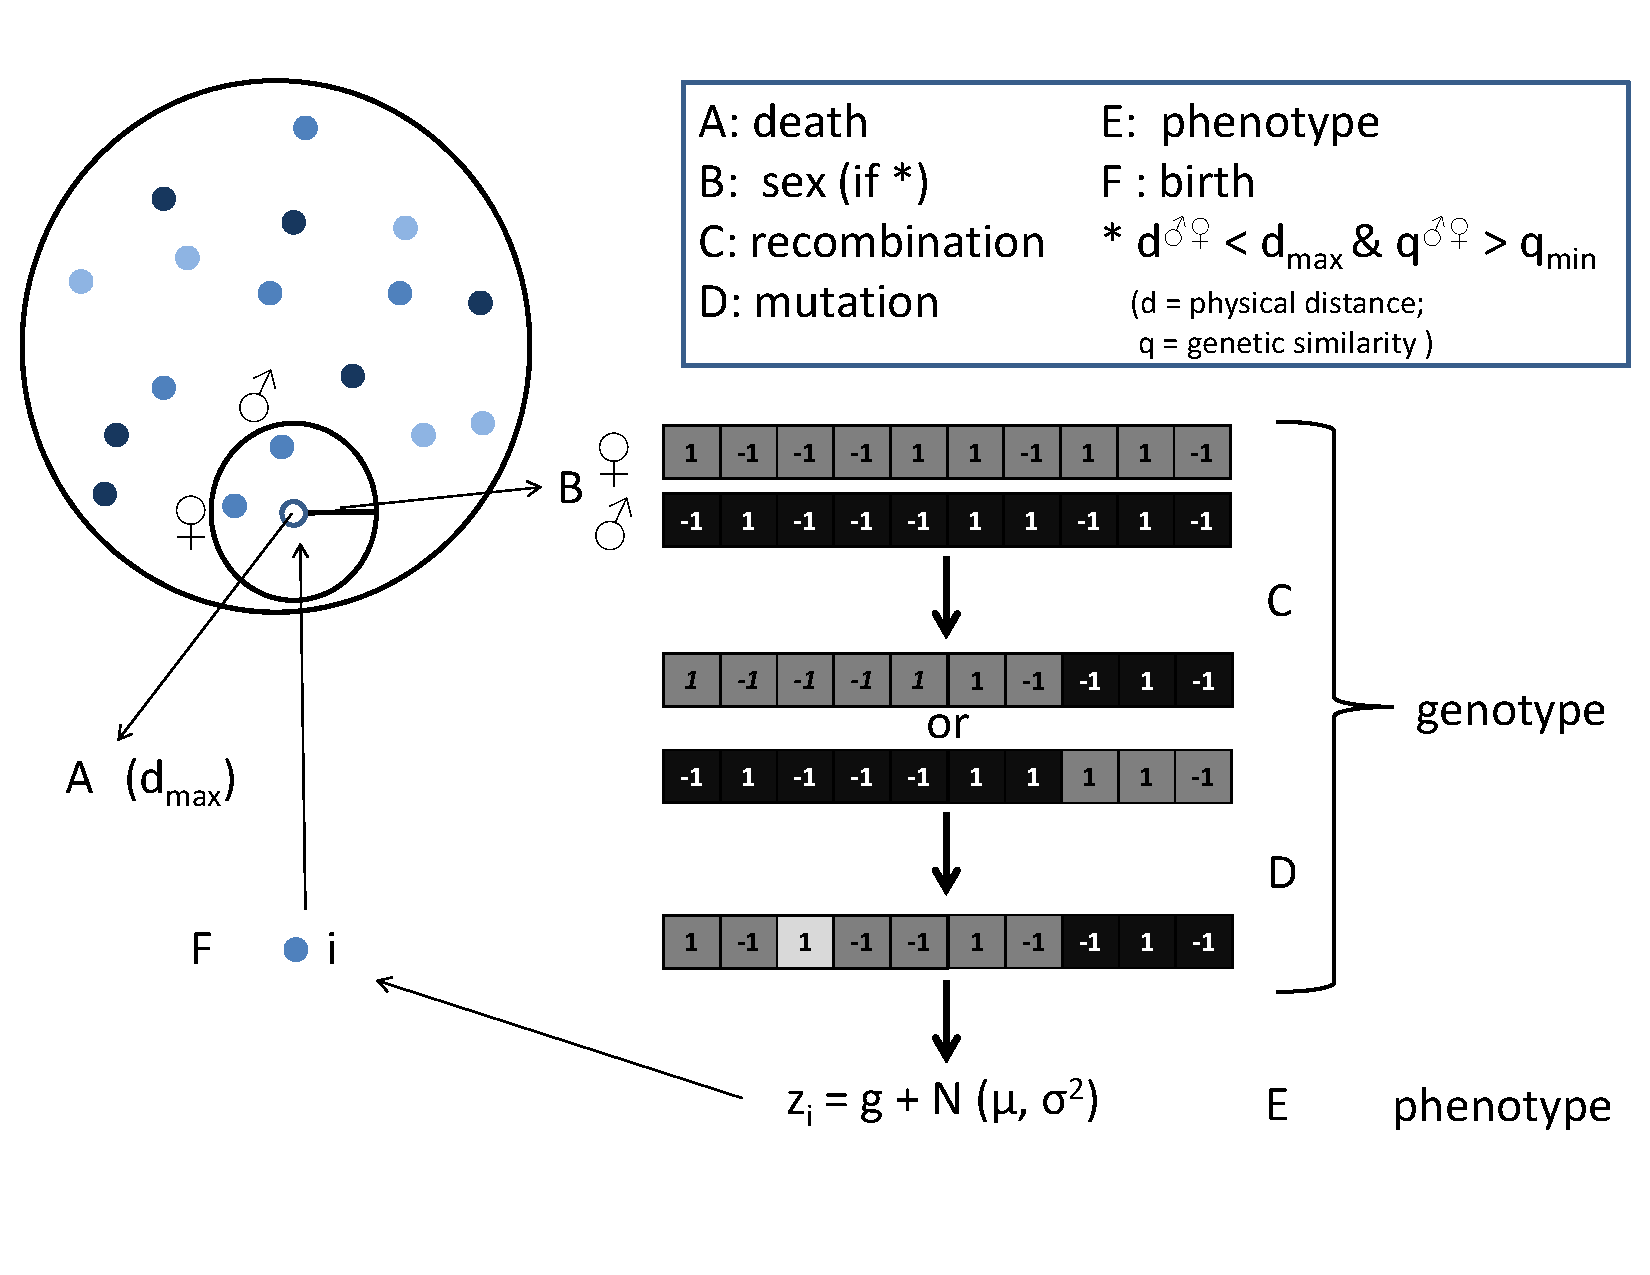
\includegraphics[scale=0.5]{Figures/IBModel6}
\par\end{centering}

\caption{This figure summarizes the death-birth cycle per time step. Individuals
are represented as filled circles and blue tones represent variation
of phenotypes. (A) an individual $k$ is randomly selected to die
and leaves an empty location in the landscape. (B) a female individual,
$\venus$, is randomly selected among all females satisfying the condition
$d_{k\venus}<d_{max}$. We then choose randomly a male, $\mars$,
among all males satisfying $d_{k\mars}<d_{max}$ and $q_{\venus\male}>q_{min}$
with $q_{min}$, the minimum genetic similarity required for mating.
In addition to these two constraints, two more are required to complete
mating. For the condition of obligate mutualism, the geographic distance
between the female (animal or plant), and an animal (or plant) individual
$j$, must satisfy $d_{j\venus}^{PA}<d_{max}^{PA}$. Finally, female
plants need the presence of an animal pollinator with a larger or
equally-sized proboscis than the corolla of the female plant, thus
individual pollinators represented as $j$, must satisfy $z_{\venus_{P}}\leq z_{j_{A}}$.
In (C) and (D) we calculate the genome of the new offspring once these
constraints are satisfied. (C) Genomes are composed of $L$ loci where
each locus can be in two allelic states ($-1,\,1$) and undergo block
crossover recombination between female (dark gray) and male (black).
A position $l$ in the genome of the parents is randomly chosen partitioning
the genome in two blocks. All genes beyond the $l$ locus in either
organism's genome is swapped between two parents and two new genomes
are formed. (D) One of the two new genomes is randomly chosen for
the offspring $i$, $S_{o}^{i}$, and it might undergo mutation (light
gray). (E) The phenotype expression of offspring $i$ is $z_{i}=g_{i}+\epsilon$
with $g_{i}=L+S_{o}^{i}$ and $\epsilon$ are the genetic and environmental
component of the phenotype, respectively. (F) The offspring $i$ occupies
the site of the dead individual $k$. \label{fig:Recombination}}


\end{figure}


\begin{figure}
\begin{centering}
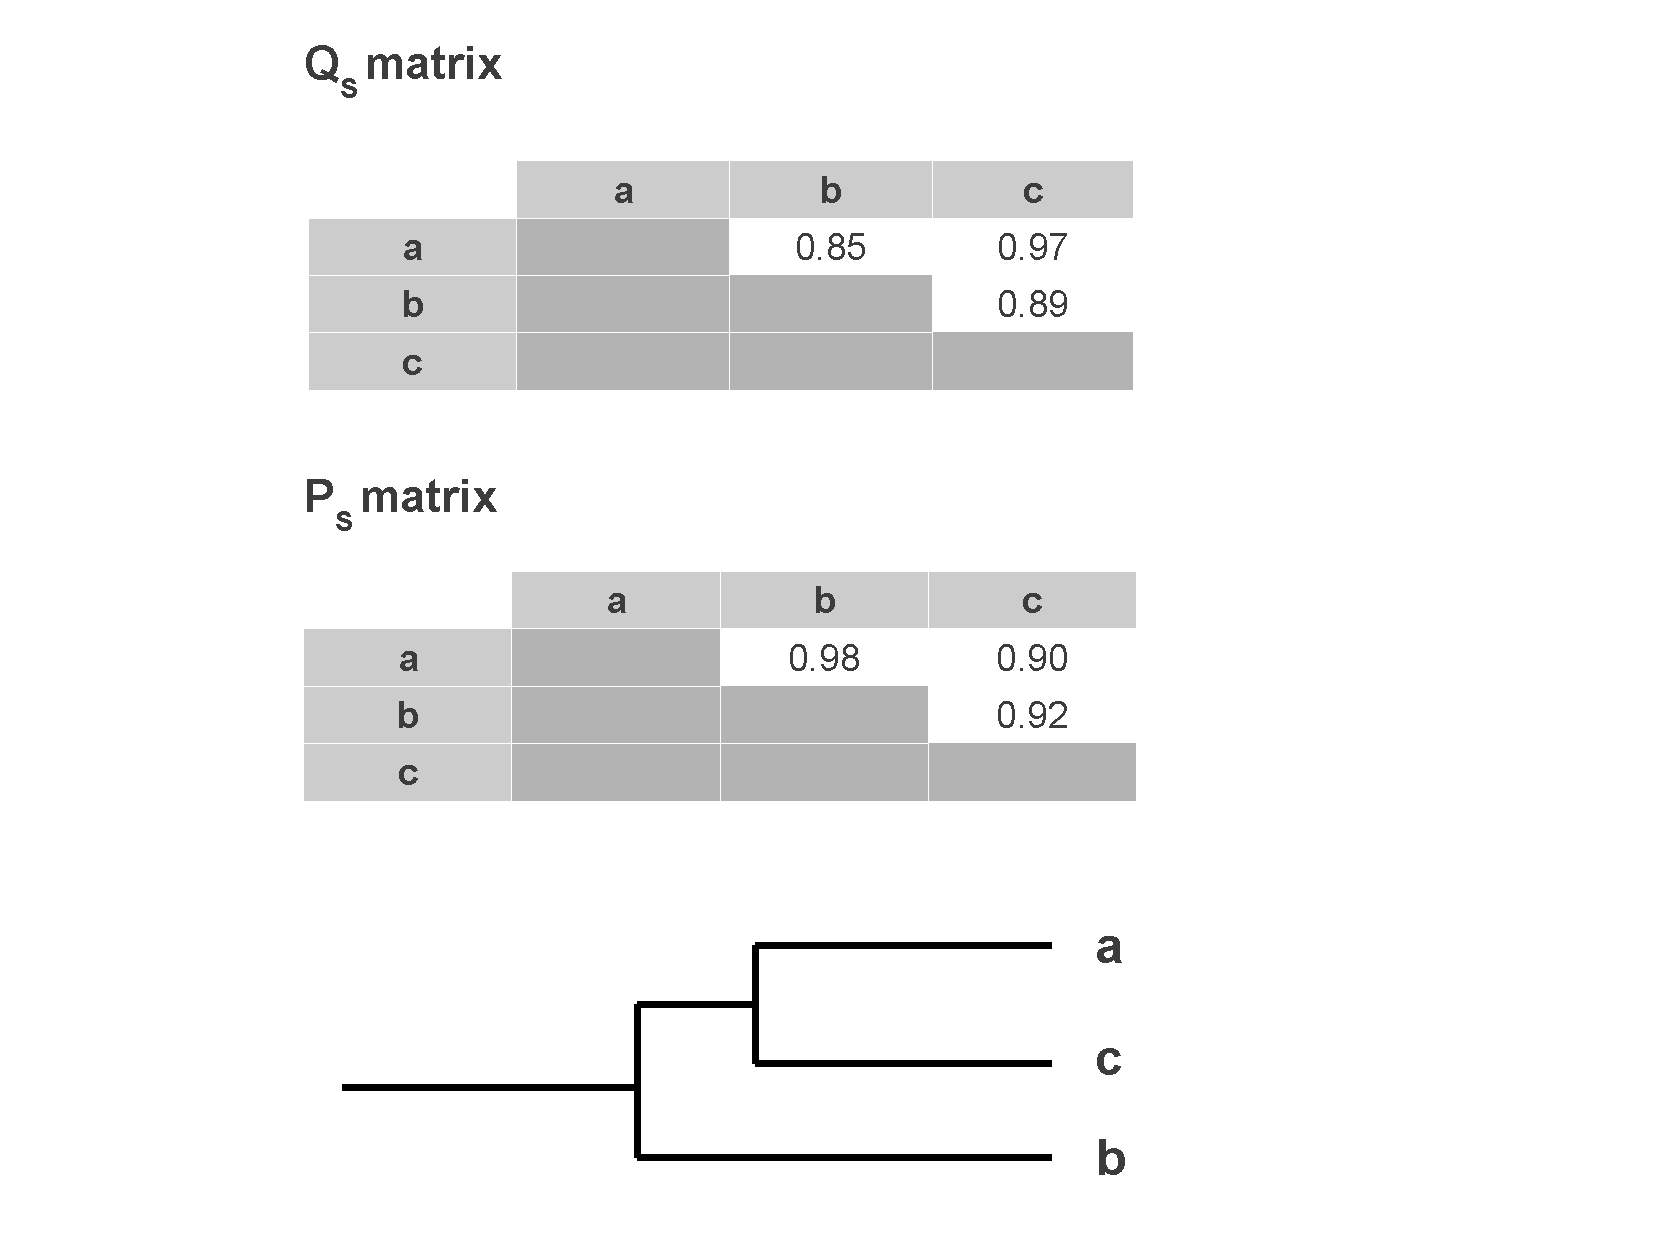
\includegraphics[scale=0.6]{Figures/convergence}
\par\end{centering}

\caption{This figure illustrates a simple example of evolutionary convergence
using species $a$, $b$ and $c$. The upper matrix ($Q_{S}=[\hat{q}_{kl}]$)
shows species $a$ and $c$ are genetically closely related, $\hat{q}_{ac}=0.97$,
while genetically distant from species $b$ ($\hat{q}_{ab}=0.85$,
$\hat{q}_{cb}=0.89$). A clear description of these genetic relationships
can be represented with a cluster tree or dendrogram, as shown in
the lower part of the figure. Thus, we establish that species $a$
and $c$ are sister species. The species phenotypic similarity matrix,
$P_{S}=[\hat{p}_{kh}]$ shows that species $a$ and $b$ are phenotypically
highly similar ($\hat{p}_{ab}=0.98$) and highly genetically dissimilar
($\hat{q}_{ab}=0.85$) (i.e. more than the average intraspecific genetic
similarity or sister species $~0.97$), indicating an event of evolutionary
convergence.\label{fig:Evolutionary-convergence}}


\end{figure}


\begin{figure}
\begin{centering}
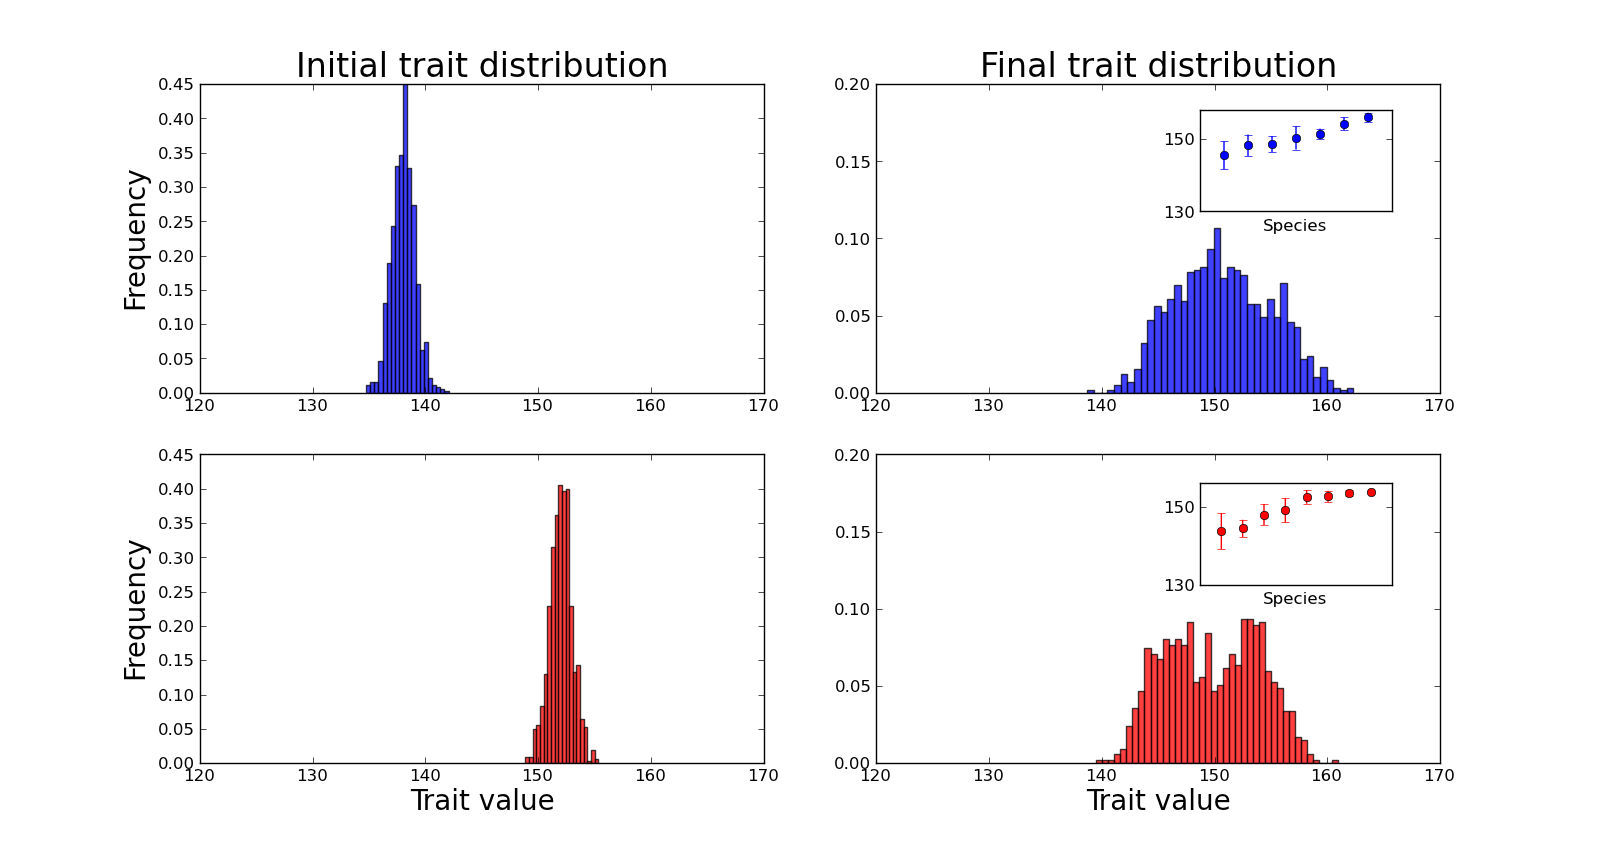
\includegraphics[scale=0.4]{Figures/trait_dist_2}
\par\end{centering}

\caption{Changes in trait distribution of plants (top, blue) and animals (bottom,
red). Left and right panels show the initial and final trait distribution,
respectively. The insets in the right panels show the mean trait and
standard error for each species sorted from the most common to the
most rare. Initial trait distributions changed towards higher variance,
and in most replicates, towards bimodal distribution in both guilds.
Plot shows the outputs from one replicate with parameters values\textbf{
$q_{min}=0.97$, $d_{max}=d_{max}^{PA}=0.3$, $\mu=5\times10^{-3}$
and $J_{P}=J_{A}=1,000$.\label{fig:Changes-in-trait}}}
\end{figure}


\begin{figure}
\begin{centering}
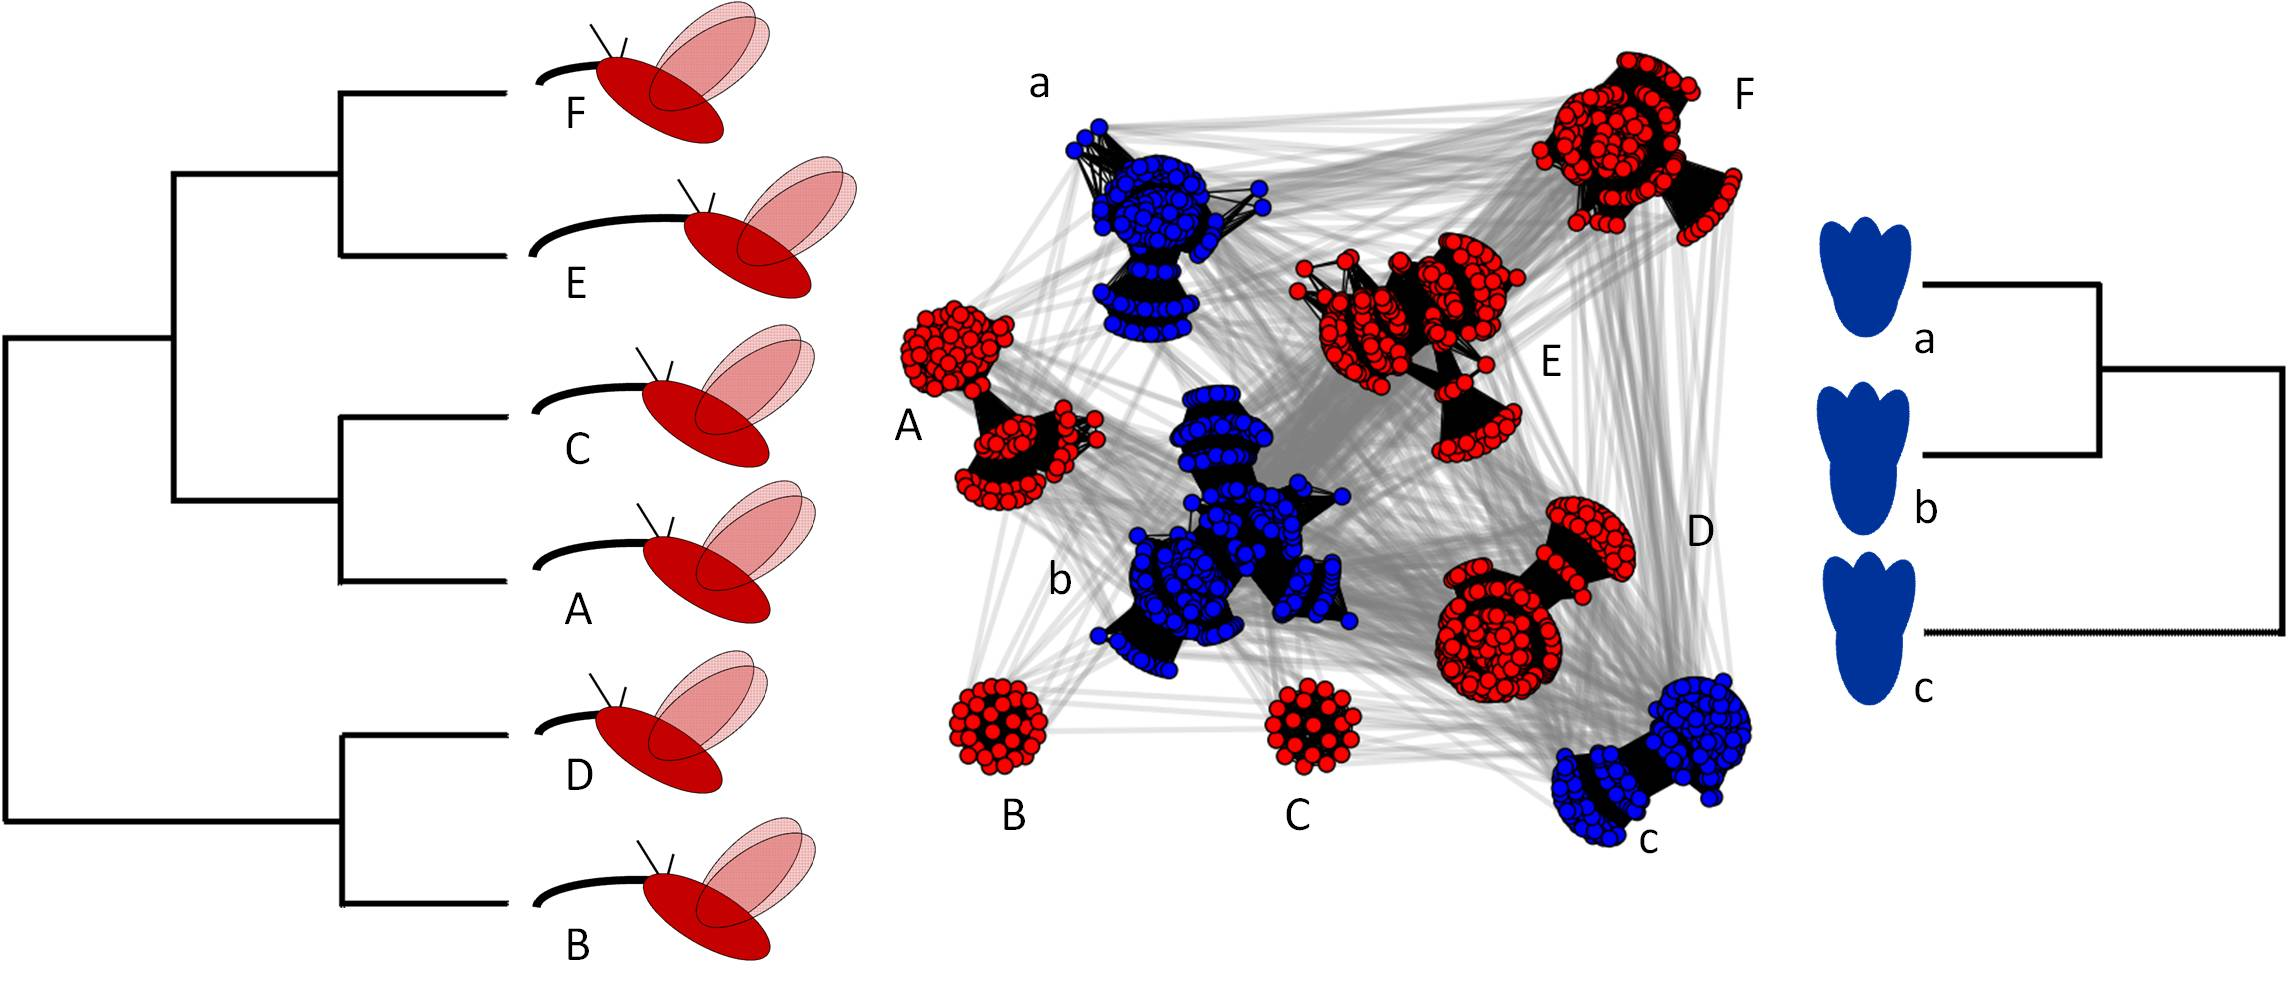
\includegraphics[scale=0.4]{Figures/ConvComp3}
\par\end{centering}

\caption{Evolutionary convergence and complementarity in plant-pollinator networks.
Trees at the left and right side show genetic similarities between
animal (red) and plant (blue) species, respectively. Mean species
trait, proboscis and corolla length, is sketched with cartoons next
to their respective position in the trees. Animals, composed by six
species, have two evolutionary convergence events (A-B and F-D). Plants,
composed by three species, have one convergent event (b-c). The central
part of the figure shows the network of plant-animal interactions,
where each node (colored filled circles) represents an individual.
The network is composed of two types of links: genetic relatedness
links (black solid) forming clusters that represent species and plant-animal
individual-based interaction links (gray). The network shows variability
in terms of genetic relatedness and plant-animal interactions within
a species (i.e. high intraspecific variability). This figure is an
example from one replicate simulation. Parameters used are as in figure
3,\textbf{ $q_{min}=0.97$, $d_{max}=d_{max}^{PA}=0.3$, $\mu=5\times10^{-3}$
and $J^{P}=J^{A}=1,000$.\label{fig:convergence-complementarity}}}


\end{figure}


\begin{figure}
\begin{centering}
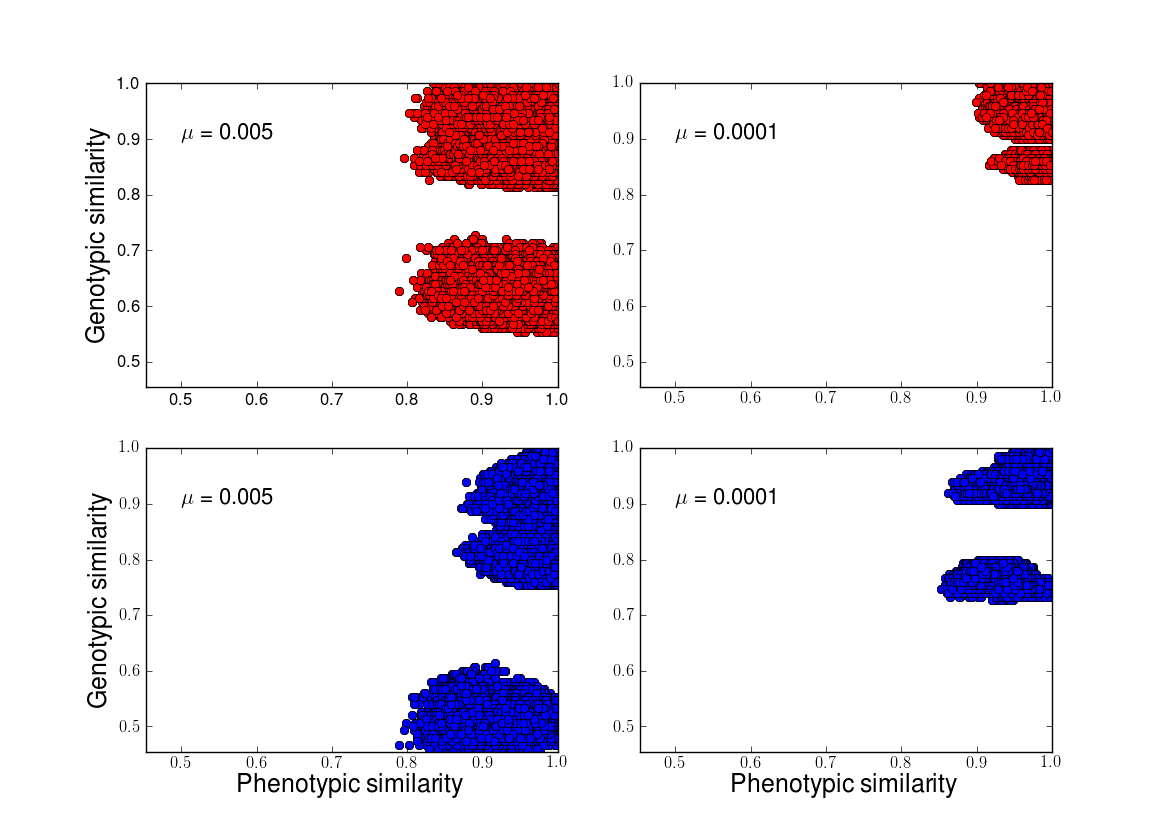
\includegraphics[scale=0.4]{Figures/phengen}
\par\end{centering}

\caption{The effect of mutation rate on the genotype-phenotype relationship.
Top and bottom panels show the genotype-phenotype relationship for
animals (red) and plants (blue), respectively. Right panels show the
genotype-phenotype relationship for mutation rate $\mu=5\times10^{-3}$
and left panels for $\mu=10^{-4}$. Each plot is a scatter plot, where
each filled circle represents phenotypic and genetic similarity between
two individuals of a particular guild (plant or animal) from one replicate.
Individuals with high phenotypic similarity and genetic dissimilarity
suggests evolutionary convergence of traits, regardless of mutation
rate. Parameters used are\textbf{ $q_{min}=0.97$, $d_{max}=d_{max}^{PA}=0.3$
}and \textbf{$J_{P}=J_{A}=1,000$. \label{fig:Genotype-phenotype-relationship-}}}
\end{figure}


\begin{figure}
\begin{centering}
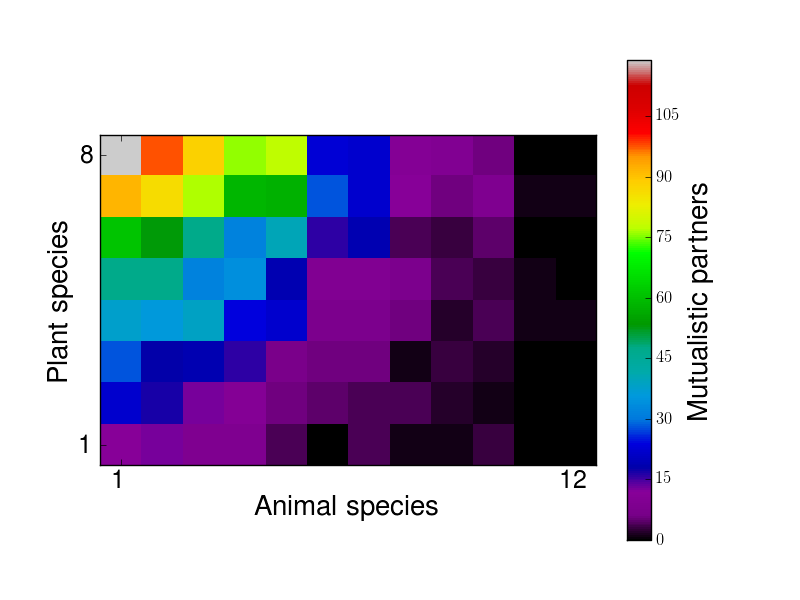
\includegraphics[scale=0.6]{Figures/matrix_plantpersp_b005_2}
\par\end{centering}

\caption{Plant-animal species interaction network. Plant species are represented
in rows and animal species in columns. The color gradient indicates
the number of mutualistic partners (i.e. individuals interacting)
shared between plant and animal species. This matrix comes from one
replicate with nine plant and thirteen animal species. The network
shows high level of nestedness ($N=0.72$) and intermediate level
of connectance ($C=0.5$). Parameters used are $q_{min}=0.97$, $d_{max}=d_{max}^{PA}=0.3$,
$\mu=5\times10^{-3}$ and $J_{P}=J_{A}=1,000$.\textbf{\label{fig:nestedness}}}


\end{figure}


\begin{figure}
\begin{centering}
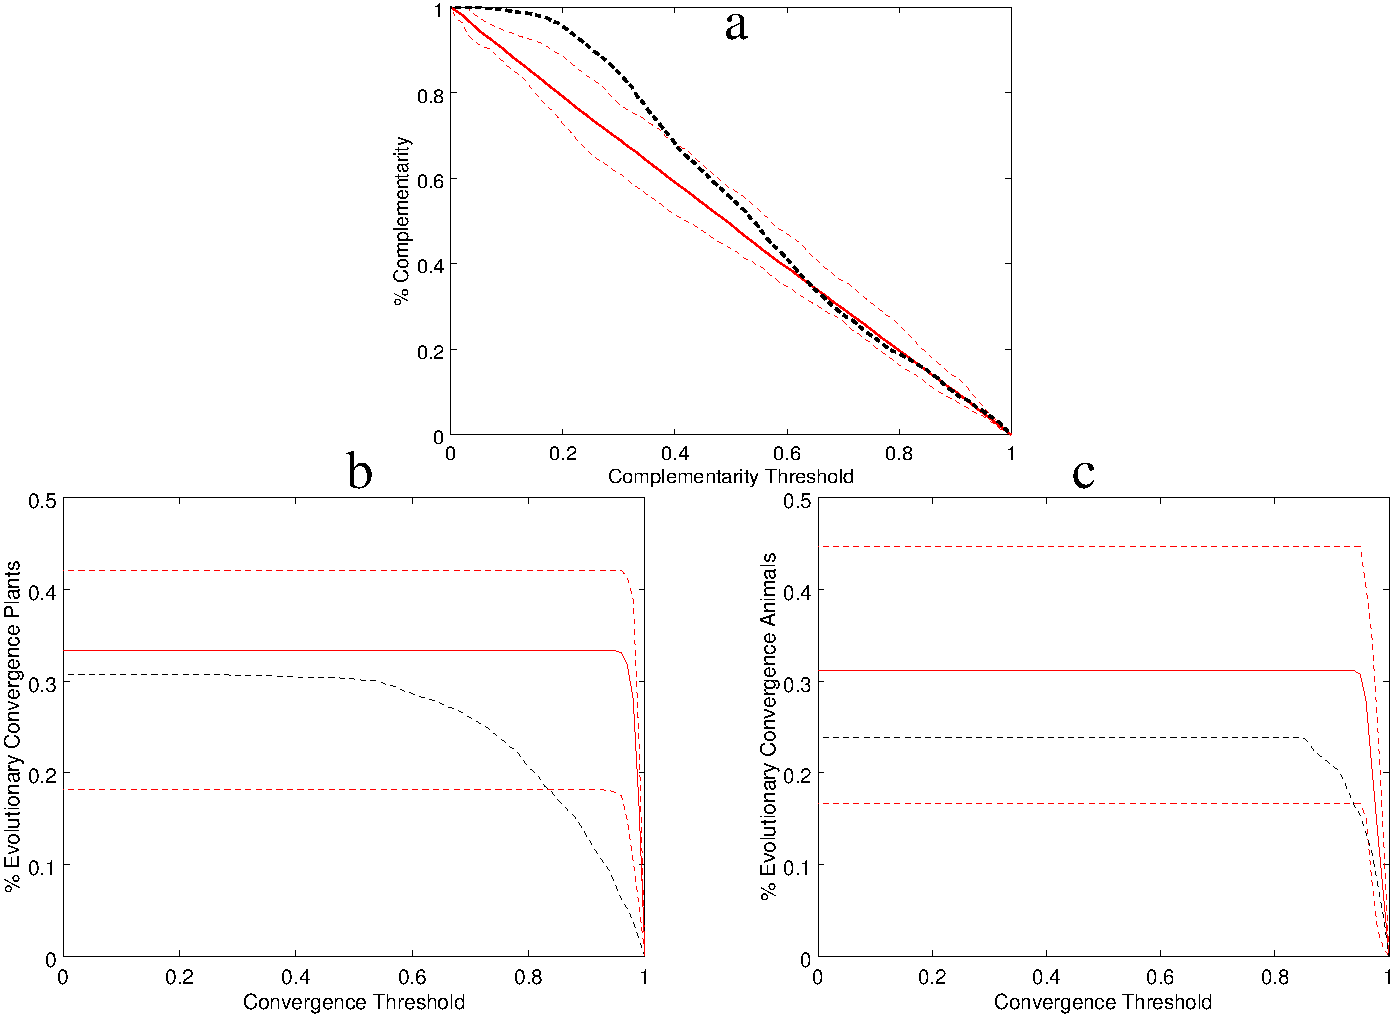
\includegraphics[scale=0.7]{Figures/compandconv-2}
\par\end{centering}

\caption{Comparison of model's predictions with estimations of convergence
and complementarity from an empirical data of a plant-pollinator community.
a) Shows the proportion of complementarity events (y-axis) as a function
of the complementarity threshold (x-axis) for the empirical data (dotted
black line) and for the model (continuous and dotted lines represent
mean, 0.05 and 0.95 CI values, respectively). Predictions are within
the CI for most complementarity threshold values. Empirical data deviates
from model predictions for complementarity values around 0.4 and lower.
b) Shows the proportion of convergence events in the plant community
(y-axis, 69 species) as a function of the convergence threshold (x-axis)
for the empirical data (dotted black line) and for the model (continuous
and dotted lines represent mean, 0.05 and 0.95 CI values, respectively).
Convergence events in the empirical data strongly deviates from model
predictions for convergence threshold values ranging between 1 and
0.82. In that range, model predicts much higher proportion of convergence
events than the empirical observations. c) Shows the proportion of
convergence events in the animal community (y-axis, 24 species) as
a function of the convergence threshold (x-axis) for the empirical
data (dotted black line) and for the model (continuous and dotted
lines represent mean, 0.05 and 0.95 CI values, respectively). Convergence
events in the empirical data are within the CI of model predictions
for most convergence threshold values. }


\end{figure}


\pagebreak{} 
\end{document}
